\documentclass[xcolor=dvipsnames]{beamer}

\usepackage{amsmath, amssymb, graphicx}
\usepackage[english]{babel}
\usepackage{times}
\usepackage[utf8]{inputenc}
\usepackage[T1]{fontenc}
\usepackage{listings}
\usepackage{hyperref}
\usepackage[norelsize,ruled,vlined]{algorithm2e}
\usepackage{color}
\usepackage{hyperref}
\usepackage{booktabs}
\usepackage{tikz}
\usetikzlibrary{matrix}
\usetikzlibrary{arrows}
\usetikzlibrary{positioning}
\usetikzlibrary{shapes.multipart}

\theoremstyle{definition}
\newtheorem{proposition}{Proposition}

\newcommand{\fancyh}{\mathcal{H}}
\newcommand{\gangle}[1]{\langle{} #1 \rangle{}}
\newcommand{\myd}{\mathrm{d}}
\newcommand{\NN}{\mathbb{N}}
\newcommand{\RR}{\mathbb{R}}
\newcommand{\ZZ}{\mathbb{Z}}

\newsavebox{\flowgraph}
\savebox{\flowgraph}{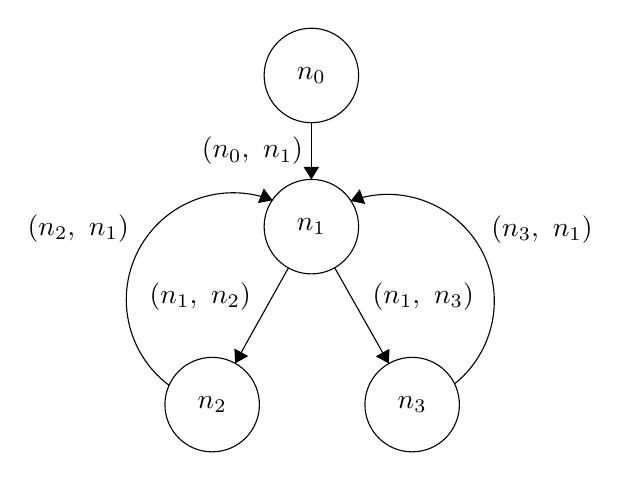
\begin{tikzpicture}[scale=0.2]
        \tikzstyle{every node}+=[inner sep=0pt]
        \draw [black] (24.7,-14) circle (3);
        \draw(24.7,-14) node {$n_0$};
        \draw [black] (24.7,-23.6) circle (3);
        \draw (24.7,-23.6) node {$n_1$};
        \draw [black] (18.4,-34.9) circle (3);
        \draw (18.4,-34.9) node {$n_2$};
        \draw [black] (31.1,-34.9) circle (3);
        \draw (31.1,-34.9) node {$n_3$};
        \draw [black] (15.682,-33.688) arc (-126.68179:-291.59948:6.793);
        \fill [black] (22.24,-21.93) -- (21.68,-21.17) -- (21.31,-22.1);
        \draw (13.14,-23.73) node [left] {$(n_2,\mbox{ }n_1)$};
        \draw [black] (27.192,-21.975) arc (110.40413:-51.35216:6.765);
        \fill [black] (27.19,-21.97) -- (28.12,-22.16) -- (27.77,-21.23);
        \draw (36.1,-23.76) node [right] {$(n_3,\mbox{ }n_1)$};
        \draw [black] (23.24,-26.22) -- (19.86,-32.28);
        \fill [black] (19.86,-32.28) -- (20.69,-31.82) -- (19.81,-31.34);
        \draw (20.89,-28.05) node [left] {$(n_1,\mbox{ }n_2)$};
        \draw [black] (26.18,-26.21) -- (29.62,-32.29);
        \fill [black] (29.62,-32.29) -- (29.66,-31.35) -- (28.79,-31.84);
        \draw (28.56,-28.03) node [right] {$(n_1,\mbox{ }n_3)$};
        \draw [black] (24.7,-17) -- (24.7,-20.6);
        \fill [black] (24.7,-20.6) -- (25.2,-19.8) -- (24.2,-19.8);
        \draw (24.2,-18.8) node [left] {$(n_0,\mbox{ }n_1)$};
    \end{tikzpicture}
}

\mode<presentation>
{% \setbeamertemplate{navigation symbols}{}
    % \setbeamertemplate{items}[ball]
    % \setbeamertemplate{blocks}[rounded][shadow=true]
    \beamertemplatenavigationsymbolsempty
    \usecolortheme[named=Sepia]{structure}
    \usetheme{Warsaw}
    \useoutertheme{infolines}
    \setbeamercovered{transparent}
}

\lstset{language = [LaTeX]TeX,
    % captionpos=b,
    basicstyle= \small \ttfamily,
    keywordstyle = \bfseries \color{blue},
    commentstyle = \color{green}
}

\definecolor{mygreen}{rgb}{0, 178, 115}

\tikzstyle{block} = [rectangle, draw, font=\tiny, text centered, rounded corners, minimum height=1em, node distance=1.5cm, minimum width=2em]
\tikzstyle{line} = [draw, -latex']
\tikzstyle{value} = [label, black, font=\tiny, thick, node distance=0.4cm]

\title[Monotone Data Flow Analysis Frameworks]{Monotone Data Flow Analysis Frameworks\\
{\small John B. Kam and Jeffrey D. Ullman, March 24th 1975}
}
\author{Fengyun Liu, Ólafur Páll Geirsson}
\institute[EPFL]{}
\date{\today}


% Delete this, if you do not want the table of contents to pop up at
% the beginning of each subsection:
\AtBeginSection[]
{\begin{frame}<beamer>{Overview}
        \tableofcontents[
            sections={1-6},
            currentsection,
            currentsubsection,
            hideothersubsections,
            sectionstyle=show/shaded,
        subsectionstyle=show/shaded/hide]
    \end{frame}
}

\begin{document}


%%%%%%%%%%%%%%%%%%%%%%%%%%%%%%%%%%%%%%%%%%%%%%%%%%%%%%%%%%%%%%%
% 0. Titlepage
%%%%%%%%%%%%%%%%%%%%%%%%%%%%%%%%%%%%%%%%%%%%%%%%%%%%%%%%%%%%%%%
\begin{frame}
    \titlepage{}
\end{frame}
\begin{frame}{Today's agenda}
\tableofcontents[hideallsubsections,
    sections={1-6}
]
\end{frame}

%%%%%%%%%%%%%%%%%%%%%%%%%%%%%%%%%%%%%%%%%%%%%%%%%%%%%%%%%%%%%%%
% 1. Background
%%%%%%%%%%%%%%%%%%%%%%%%%%%%%%%%%%%%%%%%%%%%%%%%%%%%%%%%%%%%%%%
\section{Introduction} % (fold)
\section{Background} % (fold)
\label{sec:Background}

\subsection{Flow graph}\label{sec:flowgraph}
\begin{frame}[fragile]
    \frametitle{Flow graph}
    \begin{definition}
        A flow graph is a triple \alert{$G = (N, E, n_0)$}.
    \end{definition}
    \begin{columns}
        \begin{column}{0.3\textwidth}
            Example:
            $N = \{n_0, n_1, n_2, n_3\}$
            $E = \{(n_0, n_1)$,\\
            $(n_1, n_2),(n_1, n_3)$, $(n_2, n_1),(n_3, n_1)\}$
        \end{column}
        \begin{column}{0.7\textwidth}
            \begin{center}
                \usebox{\flowgraph}
            \end{center}
        \end{column}
    \end{columns}
\end{frame}
\subsection{Semilattice}
\begin{frame}[fragile]
    \frametitle{Set $L$ with \emph{meet} operation $\wedge$}
    \begin{align*}
        a \wedge a & = a & (idempotent) \\
        a \wedge b & = b \wedge a & (commutative) \\
        a \wedge (b \wedge c) & = (a \wedge b) \wedge c & (associative)
    \end{align*}
\end{frame}
\subsection{Semilattice: ordering}
\begin{frame}[fragile]
    \frametitle{The meet $\wedge$ defines an \emph{order} on $L$}
    \begin{align*}
        a & \geqq b & \text{iff } a \wedge b = b \\
        a > b & = b \wedge a & \text{iff } a \wedge b = b \text{\ and } a \neq b
    \end{align*}
\end{frame}
\subsection{Semilattice: 0 and 1}
\begin{frame}[fragile]
    \frametitle{}
    \begin{definition}
        Element $e \in L$ is called \alert{zero}, labeled 0, if
        \[
            e \wedge x = e \qquad \forall x \in L
        \]
    \end{definition}
    Analogous to $\bot$ from last lecture.
    \pause
    \begin{definition}
        Element $e \in L$ is called \alert{one}, labeled 1, if
        \[
            e \wedge x = x \qquad \forall x \in L
        \]
    \end{definition}
    Analogous to $\top$ from last lecture.
    \pause
    \begin{block}{Example}
        $L = \{1,2\}$\\
        $A \wedge B = A \cap B$

        Example 0: $\{\}$\\
        Example 1: $\{1, 2\}$
    \end{block}
\end{frame}
\subsection{Semilattice: bounded chains}
\begin{frame}[fragile]
    \frametitle{}
    \begin{definition}
        A sequence $x_1, x_2, \ldots, x_n$ forms a \alert{chain} if $x_i > x_{i + 1}$ for $1 \leqq i < n$.
    \end{definition}
    \pause
    \begin{definition}
        The set $L$ is said to be \alert{bounded} if for each $x \in L$ there is a constant $b_x$ such that each chain beginning with $x$ has length at most $b_x$.
    \end{definition}
    \pause
    \begin{block}{Example}
        $L = \{1,2\}$\\
        $A \wedge B = A \cap B$

        Example chain: $\{1, 2\}, \{1\}, \{\}$\\
        Any finite set is bounded. Can infinite sets be bounded?
    \end{block}
\end{frame}

%%%%%%%%%%%%%%%%%%%%%%%%%%%%%%%%%%%%%%%%%%%%%%%%%%%%%%%%%%%%%%%
% 2. Monotone Data Flow Analysis Frameworks
%%%%%%%%%%%%%%%%%%%%%%%%%%%%%%%%%%%%%%%%%%%%%%%%%%%%%%%%%%%%%%%
\section{Monotone Data Flow Analysis Frameworks} % (fold)
\label{sec:mdfaf}
\subsection{Monotone function space}
\begin{frame}[fragile]
    \frametitle{Monotone function space}
    \begin{definition}
        Given a bounded semilattice $L$, a set of functions $F$ on $L$ is said
        to be a \alert{monotone function space} associated with $L$ if the
        following conditions are satisfied:
        \begin{enumerate}
            \item[M1] Each $f \in F$ satisfies the \emph{monotonicity condition} if for all $x, y \in L$,
                \[
                    f (x \wedge y) \leqq f(x) \wedge f(y)
                \]
            \item[M2] There exists an identity function $i$ in $F$.
            \item[M3] $F$ is closed under composition.
            \item[M4] $L$ is equal to the closure of $\{0\}$ under the meet
                operation and application of functions in $F$ (more on next slide).
        \end{enumerate}
    \end{definition}
\end{frame}
\begin{frame}[fragile]
    \frametitle{Monotone function space (M4)}
    \begin{definition}
        \begin{enumerate}
            \item[M4] $L$ is equal to the closure of $\{0\}$ under the meet
                operation and application of functions in $F$.
        \end{enumerate}
    \end{definition}
    \begin{itemize}
        \item Read: given $F$, $\{0\}$ and the meet operation, we can generate
            all elements of $L$.
        \item Alternatively: Any element in $L$ can be expressed as a sequence
            of applications of functions in $F$ and the meet operation with
            $\{0\}$.
    \end{itemize}

\end{frame}

\subsection{Monotone data flow analysis framework}
\begin{frame}[fragile]
    \frametitle{Monotone data flow analysis framework}
    \begin{definition}
        A Monotone data flow analysis framework (from here on \emph{framework}) is a triple \alert{$D = (L, \wedge, F)$}, where
        \begin{enumerate}[(1)]
            \item $L$ is a bounded semilattice with meet $\wedge$
            \item $F$ is a monotone function space associated with $L$
        \end{enumerate}
    \end{definition}
\end{frame}

\begin{frame}[fragile]
    \frametitle{Framework instance}
    \begin{definition}
        A particular instance of a framework is a pair \alert{$I = (G, M)$}, where
        \begin{enumerate}[(1)]
            \item $G = (N, E, n_0)$ is a flow graph.
            \item $M: N \rightarrow F$ is a function which maps each node in $N$ to a function in $F$.
        \end{enumerate}
    \end{definition}
\end{frame}
\begin{frame}[fragile]
    \frametitle{Putting it together}
    \begin{columns}
        \begin{column}{0.4\textwidth}
            \begin{itemize}
                \item Instance $I = (G, M)$
                \item Framework $D = (L, \wedge, F)$
                \item $M: N \rightarrow F$
                \item $F: L \rightarrow L$
                \item $\wedge: L \times L \rightarrow L$
            \end{itemize}
        \end{column}
        \begin{column}{0.6\textwidth}
            \begin{center}
                \usebox{\flowgraph}
            \end{center}
        \end{column}
    \end{columns}
\end{frame}
\subsection{Constant propagation}
\begin{frame}[fragile]
    \frametitle{Constant propagation}
    Constant propagation can be formalized as a monotone data flow analysis framework where
    \begin{align*}
        CONST  & = (L, \wedge, F) & \text{framework}\\
        V      & = \{A_1, A_2, \ldots \} & \text{infinite set of variables} \\
        L      & \subset 2^{V \times \RR} & \text{possible variable assignments}\\
        \wedge & = \text{set intersection}
    \end{align*}
\end{frame}
\begin{frame}[fragile]
    \frametitle{Constant propagation is not distributive}
    \begin{definition}
        For all $x, y \in L$ and $f \in F$, \alert{distributivity} is satisfied when
        \begin{equation*}
            f(x \wedge y) = f(x) \wedge f(y)
        \end{equation*}
    \end{definition}
    \begin{columns}
        \begin{column}{0.4\textwidth}
            \begin{itemize}
                \item $f(x \wedge y) =$ \\$\{(A, 2), (B, 3)\} \cap \{(A, 3), (B, 2)\} = \emptyset$
                \item $f(x) \wedge f(y) =$ \\$\{(A, 2), (B, 3), (C, 5)\} \cap \{(A, 3), (B, 2), (C, 5)\} = \{(C, 5)\}$
            \end{itemize}
        \end{column}
        \begin{column}{0.6\textwidth}
            \begin{figure}
                \newcommand{\ndistance}{0.8cm}
                \centering
                \begin{tikzpicture}[node distance = 1cm, auto, every text node part/.style={align=left}]
                    % Place nodes
                    \node [block, label=above:] (n0) {$i$};
                    \node [value, right of=n0, node distance=0.8cm] (s0) {};
                    \node [block, below of=n0, label=above:, xshift=-0.8cm, node distance = \ndistance] (n1) {$A = 2$\\$B = 3$};
                    \node [value, left of=n1, node distance=1.5cm] (s1) {$z = \{(A, 2), (B, 3)\}$};
                    \node [block, below of=n0, label=above:, xshift=0.8cm,  node distance = \ndistance] (n2) {$A = 3$\\$B = 2$};
                    \node [value, right of=n2, node distance=1.5cm] (s2) {$z' = \{(A, 3), (B, 2)\}$};
                    \node [block, below of=n1, label=130:, xshift=0.85cm, node distance = \ndistance] (n3) {$C = A + B$};
                    \node [value, right of=n3, node distance=0.8cm] (s3) {};
                    \node [block, below of=n3, label=100:, node distance = \ndistance] (n4) {};
                    \node [value, right of=n4, node distance=0.5cm] (s3) {};
                    % Draw edges
                    \path [line] (n0) -- (n1);
                    \path [line] (n0) -- (n2);
                    \path [line] (n1) -- (n3);
                    \path [line] (n2) -- (n3);
                    \path [line] (n3) -- (n4);
                \end{tikzpicture}
                \caption{Counter example to distributivity of CONST}
            \end{figure}
        \end{column}
    \end{columns}
\end{frame}

% section Monotone Data Flow Analysis Frameworks (end)
%%%%%%%%%%%%%%%%%%%%%%%%%%%%%%%%%%%%%%%%%%%%%%%%%%%%%%%%%%%%%%%
% 3. Approaches to solving Monotone Data Flow Analysis Frameworks
%%%%%%%%%%%%%%%%%%%%%%%%%%%%%%%%%%%%%%%%%%%%%%%%%%%%%%%%%%%%%%%
\section{Approaches to solving monotone frameworks} % (fold)
\label{sec:approaches}
\subsection{Algorithm 1 (Kildall's Algorithm)}
\begin{frame}[fragile]
    \frametitle{Algorithm 1}

\end{frame}

% section approaches
%%%%%%%%%%%%%%%%%%%%%%%%%%%%%%%%%%%%%%%%%%%%%%%%%%%%%%%%%%%%%%%
% 4. A Variant of Kildall's Algorithm
%%%%%%%%%%%%%%%%%%%%%%%%%%%%%%%%%%%%%%%%%%%%%%%%%%%%%%%%%%%%%%%
\section{A Variant of Kildall's Algorithm} % (fold)
\label{sec:variant}

% section A Variant of Kildall's Algorithm


\subsection{Algorithm 2}

\begin{frame}
  \frametitle{Initialization}

  \begin{columns}[onlytextwidth]
    \begin{column}{0.55\textwidth}
      \begin{equation*}
        B[n] =
        \begin{cases}
          f_{n_0}(0) & \text{if } n = n_0\\
          1 & otherwise
        \end{cases}
      \end{equation*}

      \begin{itemize}
      % \item \textit{Initialization}
      \item 0 - zero element of the lattice
      \item 1 - one element of the lattice
      \item $i$ - identity function
      \item $f_{n_0}$ - the function that $n_0$ corresponds to
      \item $L \subset 2^{V \times \RR}$ where $V = \{A, B, C\}$
      \end{itemize}
    \end{column}

    \begin{column}{0.45\textwidth}
        \begin{center}
            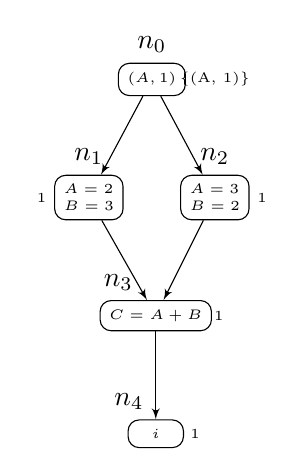
\begin{tikzpicture}[node distance = 2cm, auto, every text node part/.style={align=left}]
            % Place nodes
            \node [block, label=above:$n_0$] (n0) {$(A, 1)$};
            \node [value, right of=n0, node distance=0.8cm] (s0) {\{(A, 1)\}};
            \node [block, below of=n0, label=above:$n_1$, xshift=-0.8cm] (n1) {$A = 2$\\$B = 3$};
            \node [value, left of=n1, node distance=0.6cm] (s1) {1};
            \node [block, below of=n0, label=above:$n_2$, xshift=0.8cm] (n2) {$A = 3$\\$B = 2$};
            \node [value, right of=n2, node distance=0.6cm] (s2) {1};
            \node [block, below of=n1, label=130:$n_3$, xshift=0.85cm] (n3) {$C = A + B$};
            \node [value, right of=n3, node distance=0.8cm] (s3) {1};
            \node [block, below of=n3, label=100:$n_4$] (n4) {$i$};
            \node [value, right of=n4, node distance=0.5cm] (s3) {1};
            % Draw edges
            \path [line] (n0) -- (n1);
            \path [line] (n0) -- (n2);
            \path [line] (n1) -- (n3);
            \path [line] (n2) -- (n3);
            \path [line] (n3) -- (n4);
            \end{tikzpicture}
        \end{center}
    \end{column}
  \end{columns}
\end{frame}

\begin{frame}
  \frametitle{Iteration Step}
  \begin{columns}[onlytextwidth]
    \begin{column}{0.55\textwidth}
      Visit nodes other than $n_0$ in order $v_1, v_2, ...$, for each visited node $n$, set \\
      \begin{equation*}
        B[n] = \bigwedge_{p \in PRED(n)} f_n(B[p])
      \end{equation*}

      Conditions of the sequence($v_1, v_2, ...$):
      \begin{itemize}
      \item If a node doesn't satisfy the equation above, it should be visited again.
      \item If all nodes satisfy the equation, the sequence eventually end.
      \end{itemize}

      \only<1>{
        Example: \alert{$n_2, n_1, n_3, n_2, n_3$}
      }

    \end{column}

    \begin{column}{0.45\textwidth}
      \begin{center}
        \only<1>{
          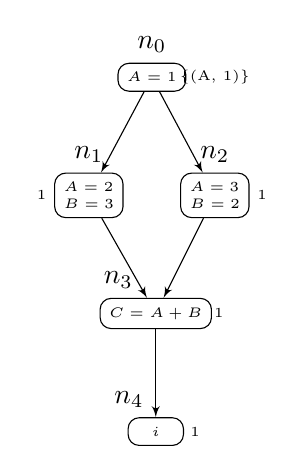
\begin{tikzpicture}[node distance = 2cm, auto, every text node part/.style={align=left}]
            % Place nodes
            \node [block, label=above:$n_0$] (n0) {$A = 1$};
            \node [value, right of=n0, node distance=0.8cm] (s0) {\{(A, 1)\}};
            \node [block, below of=n0, label=above:$n_1$, xshift=-0.8cm] (n1) {$A = 2$\\$B = 3$};
            \node [value, left of=n1, node distance=0.6cm] (s1) {1};
            \node [block, below of=n0, label=above:$n_2$, xshift=0.8cm] (n2) {$A = 3$\\$B = 2$};
            \node [value, right of=n2, node distance=0.6cm] (s2) {1};
            \node [block, below of=n1, label=130:$n_3$, xshift=0.85cm] (n3) {$C = A + B$};
            \node [value, right of=n3, node distance=0.8cm] (s3) {1};
            \node [block, below of=n3, label=100:$n_4$] (n4) {$i$};
            \node [value, right of=n4, node distance=0.5cm] (s3) {1};
            % Draw edges
            \path [line] (n0) -- (n1);
            \path [line] (n0) -- (n2);
            \path [line] (n1) -- (n3);
            \path [line] (n2) -- (n3);
            \path [line] (n3) -- (n4);
          \end{tikzpicture}
        }
        \only<2>{
          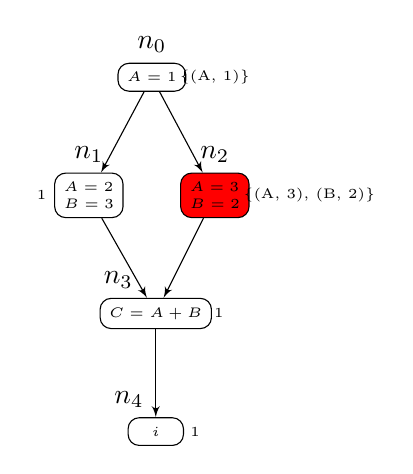
\begin{tikzpicture}[node distance = 2cm, auto, every text node part/.style={align=left}]
            % Place nodes
            \node [block, label=above:$n_0$] (n0) {$A = 1$};
            \node [value, right of=n0, node distance=0.8cm] (s0) {\{(A, 1)\}};
            \node [block, below of=n0, label=above:$n_1$, xshift=-0.8cm] (n1) {$A = 2$\\$B = 3$};
            \node [value, left of=n1, node distance=0.6cm] (s1) {1};
            \node [block, fill=red, below of=n0, label=above:$n_2$, xshift=0.8cm] (n2) {$A = 3$\\$B = 2$};
            \node [value, right of=n2, node distance=1.2cm] (s2) {\{(A, 3), (B, 2)\}};
            \node [block, below of=n1, label=130:$n_3$, xshift=0.85cm] (n3) {$C = A + B$};
            \node [value, right of=n3, node distance=0.8cm] (s3) {1};
            \node [block, below of=n3, label=100:$n_4$] (n4) {$i$};
            \node [value, right of=n4, node distance=0.5cm] (s3) {1};
            % Draw edges
            \path [line] (n0) -- (n1);
            \path [line] (n0) -- (n2);
            \path [line] (n1) -- (n3);
            \path [line] (n2) -- (n3);
            \path [line] (n3) -- (n4);
          \end{tikzpicture}

          \alert{$n_2$}, $n_1, n_3, n_2, n_4$
        }
        \only<3>{
          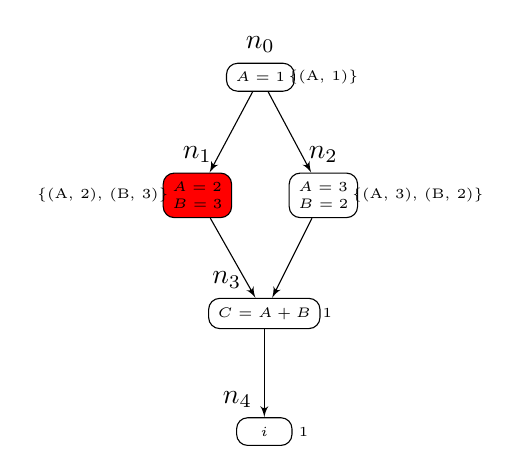
\begin{tikzpicture}[node distance = 2cm, auto, every text node part/.style={align=left}]
            % Place nodes
            \node [block, label=above:$n_0$] (n0) {$A = 1$};
            \node [value, right of=n0, node distance=0.8cm] (s0) {\{(A, 1)\}};
            \node [block, fill=red, below of=n0, label=above:$n_1$, xshift=-0.8cm] (n1) {$A = 2$\\$B = 3$};
            \node [value, left of=n1, node distance=1.2cm] (s1) {\{(A, 2), (B, 3)\}};
            \node [block, below of=n0, label=above:$n_2$, xshift=0.8cm] (n2) {$A = 3$\\$B = 2$};
            \node [value, right of=n2, node distance=1.2cm] (s2) {\{(A, 3), (B, 2)\}};
            \node [block, below of=n1, label=130:$n_3$, xshift=0.85cm] (n3) {$C = A + B$};
            \node [value, right of=n3, node distance=0.8cm] (s3) {1};
            \node [block, below of=n3, label=100:$n_4$] (n4) {$i$};
            \node [value, right of=n4, node distance=0.5cm] (s3) {1};
            % Draw edges
            \path [line] (n0) -- (n1);
            \path [line] (n0) -- (n2);
            \path [line] (n1) -- (n3);
            \path [line] (n2) -- (n3);
            \path [line] (n3) -- (n4);
          \end{tikzpicture}

          $n_2$, \alert{$n_1$}, $n_3, n_2, n_4$
        }
        \only<4>{
          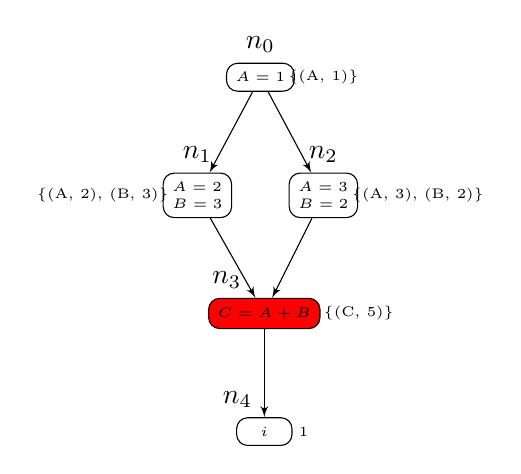
\begin{tikzpicture}[node distance = 2cm, auto, every text node part/.style={align=left}]
            % Place nodes
            \node [block, label=above:$n_0$] (n0) {$A = 1$};
            \node [value, right of=n0, node distance=0.8cm] (s0) {\{(A, 1)\}};
            \node [block, below of=n0, label=above:$n_1$, xshift=-0.8cm] (n1) {$A = 2$\\$B = 3$};
            \node [value, left of=n1, node distance=1.2cm] (s1) {\{(A, 2), (B, 3)\}};
            \node [block, below of=n0, label=above:$n_2$, xshift=0.8cm] (n2) {$A = 3$\\$B = 2$};
            \node [value, right of=n2, node distance=1.2cm] (s2) {\{(A, 3), (B, 2)\}};
            \node [block, fill=red, below of=n1, label=130:$n_3$, xshift=0.85cm] (n3) {$C = A + B$};
            \node [value, right of=n3, node distance=1.2cm] (s3) {\{(C, 5)\}};
            \node [block, below of=n3, label=100:$n_4$] (n4) {$i$};
            \node [value, right of=n4, node distance=0.5cm] (s3) {1};
            % Draw edges
            \path [line] (n0) -- (n1);
            \path [line] (n0) -- (n2);
            \path [line] (n1) -- (n3);
            \path [line] (n2) -- (n3);
            \path [line] (n3) -- (n4);
          \end{tikzpicture}

          $n_2$, $n_1$, \alert{$n_3$}, $n_2, n_4$
        }
        \only<5>{
          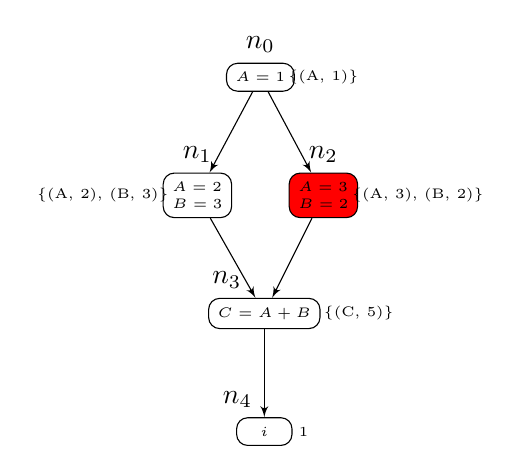
\begin{tikzpicture}[node distance = 2cm, auto, every text node part/.style={align=left}]
            % Place nodes
            \node [block, label=above:$n_0$] (n0) {$A = 1$};
            \node [value, right of=n0, node distance=0.8cm] (s0) {\{(A, 1)\}};
            \node [block, below of=n0, label=above:$n_1$, xshift=-0.8cm] (n1) {$A = 2$\\$B = 3$};
            \node [value, left of=n1, node distance=1.2cm] (s1) {\{(A, 2), (B, 3)\}};
            \node [block, fill=red, below of=n0, label=above:$n_2$, xshift=0.8cm] (n2) {$A = 3$\\$B = 2$};
            \node [value, right of=n2, node distance=1.2cm] (s2) {\{(A, 3), (B, 2)\}};
            \node [block, below of=n1, label=130:$n_3$, xshift=0.85cm] (n3) {$C = A + B$};
            \node [value, right of=n3, node distance=1.2cm] (s3) {\{(C, 5)\}};
            \node [block, below of=n3, label=100:$n_4$] (n4) {$i$};
            \node [value, right of=n4, node distance=0.5cm] (s3) {1};
            % Draw edges
            \path [line] (n0) -- (n1);
            \path [line] (n0) -- (n2);
            \path [line] (n1) -- (n3);
            \path [line] (n2) -- (n3);
            \path [line] (n3) -- (n4);
          \end{tikzpicture}

          $n_2$, $n_1$, $n_3$, \alert{$n_2$}, $n_4$
        }
        \only<6>{
          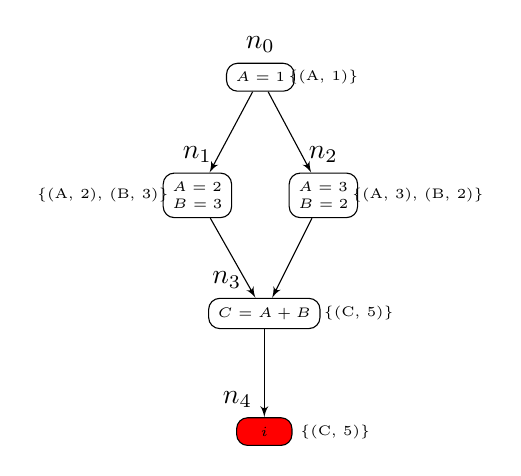
\begin{tikzpicture}[node distance = 2cm, auto, every text node part/.style={align=left}]
            % Place nodes
            \node [block, label=above:$n_0$] (n0) {$A = 1$};
            \node [value, right of=n0, node distance=0.8cm] (s0) {\{(A, 1)\}};
            \node [block, below of=n0, label=above:$n_1$, xshift=-0.8cm] (n1) {$A = 2$\\$B = 3$};
            \node [value, left of=n1, node distance=1.2cm] (s1) {\{(A, 2), (B, 3)\}};
            \node [block, below of=n0, label=above:$n_2$, xshift=0.8cm] (n2) {$A = 3$\\$B = 2$};
            \node [value, right of=n2, node distance=1.2cm] (s2) {\{(A, 3), (B, 2)\}};
            \node [block, below of=n1, label=130:$n_3$, xshift=0.85cm] (n3) {$C = A + B$};
            \node [value, right of=n3, node distance=1.2cm] (s3) {\{(C, 5)\}};
            \node [block, fill=red, below of=n3, label=100:$n_4$] (n4) {$i$};
            \node [value, right of=n4, node distance=0.9cm] (s3) {\{(C, 5)\}};
            % Draw edges
            \path [line] (n0) -- (n1);
            \path [line] (n0) -- (n2);
            \path [line] (n1) -- (n3);
            \path [line] (n2) -- (n3);
            \path [line] (n3) -- (n4);
          \end{tikzpicture}

          $n_2$, $n_1$, $n_3$, $n_2$, \alert{$n_4$}
        }
      \end{center}
    \end{column}
  \end{columns}
\end{frame}

\begin{frame}
  \frametitle{Final Step}
  \begin{columns}[onlytextwidth]
    \begin{column}{0.5\textwidth}
      For each node, set
      \begin{equation*}
        H[n] =
        \begin{cases}
          0 & \text{if } n = n_0\\
          \bigwedge_{p \in PRED(n)} B[p] & otherwise
        \end{cases}
      \end{equation*}
    \end{column}
    \begin{column}{0.5\textwidth}
      \begin{center}
        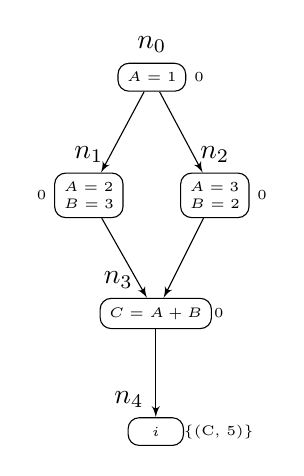
\begin{tikzpicture}[node distance = 2cm, auto, every text node part/.style={align=left}]
          % Place nodes
          \node [block, label=above:$n_0$] (n0) {$A=1$};
          \node [value, right of=n0, node distance=0.6cm] (s0) {0};
          \node [block, below of=n0, label=above:$n_1$, xshift=-0.8cm] (n1) {$A = 2$\\$B = 3$};
          \node [value, left of=n1, node distance=0.6cm] (s1) {0};
          \node [block, below of=n0, label=above:$n_2$, xshift=0.8cm] (n2) {$A = 3$\\$B = 2$};
          \node [value, right of=n2, node distance=0.6cm] (s2) {0};
          \node [block, below of=n1, label=130:$n_3$, xshift=0.85cm] (n3) {$C = A + B$};
          \node [value, right of=n3, node distance=0.8cm] (s3) {0};
          \node [block, below of=n3, label=100:$n_4$] (n4) {$i$};
          \node [value, right of=n4, node distance=0.8cm] (s3) {\{(C, 5)\}};
          % Draw edges
          \path [line] (n0) -- (n1);
          \path [line] (n0) -- (n2);
          \path [line] (n1) -- (n3);
          \path [line] (n2) -- (n3);
          \path [line] (n3) -- (n4);
        \end{tikzpicture}
      \end{center}
    \end{column}
  \end{columns}
\end{frame}

\subsection{Properties of Algorithm 2}

\begin{frame}
  \frametitle{Properties of Algorithm - Theorem 5}
  \begin{theorem}
    Given an instance $I = (G, M)$ of a framework $D = (L, \wedge, F)$ as input to Algorithm 2:

    \begin{enumerate}[(i)]
    \item Algorithm 2 will eventually halt. \alert{\scriptsize proof: B[n]
        decrease and L is bounded}.
    \item The result we get is unique independent of the order in which the
        nodes are visited. \alert{\scriptsize proof: B[n] is the  maximal fix
        point of the set of equations}.
    \item $(\forall n \in N) H[n] \leqq \bigwedge_{P \in PATH(n)}f_P(0)$.
        \alert{\scriptsize proof: Induction on the length of P}.
    \item If A[n] is the result of applying Algorithm 1 to $I = (G, M)$, then
        $A[n] \leqq H[n]$. \only<2>{\alert{Let's prove this!}}
    \end{enumerate}
  \end{theorem}
\end{frame}

\begin{frame}
  \frametitle{Property (iv) of Algorithm 2 - Proof}
  \begin{proposition}[$iv$]
      If A[n] is the result of applying Algorithm 1 to $I = (G, M)$, then $A[n] \leqq H[n]$.
  \end{proposition}

  \begin{block}{Proof by induction on steps of algorithm 2}
      For node $n_0$, the property trivially holds because $A[n] = 0 \leqq e$ for any $e \in L$. % f_0(A[n_0] = 0) = 0 \leqq B[n_0] = f_{n_0}(0)$
      For all other node $n \in N$, the proposition is equivalent to:
      \alert{$f_n(A[n]) \leqq B[n]$} because
      \begin{align*}
          A[n] & = \bigwedge_{p \in PRED(n)} f_p(A[p]) \\
          H[n] & = \bigwedge_{p \in PRED(n)} B[p]
      \end{align*}

    \emph{Base step ($m = 0$)}. $B^0[n] = 1$ and by definition $f_n(A[n]) \leqq 1$
  \end{block}
\end{frame}
\begin{frame}
    \begin{proof}[Proof by induction on steps of algorithm 2 (cont.)]
        \emph{Induction step ($m > 0$)}. Our induction hypothesis (IH) is:
        \[
            B^{m-1}[n] \leqq f_n(A[n])
        \]

      Then
      \begin{align*}
   B^m[n] & = \bigwedge_{p \in PRED(n)} f_n(B^{m-1}[p]) \\
          & = \bigwedge_{p \in PRED(n)} f_n(f_p(A[p]))  & \text{(monotonicity \& IH)} \\
          & \leqq f_n(\bigwedge_{p \in PRED(n)} f_p(A[p])) & \text{(monotonicity)} \\
          & =  f_n(A[n])
      \end{align*}
  \end{proof}
\end{frame}

\subsection{Algorithm 2 is not Universal}

\begin{frame}
  \frametitle{Infinite number of counterexamples}
  For the following constructed graph, for node $n$ we have:

  \[
      MOP = \bigwedge_{P \in PATH(n)}f_P(0) \leqq f(x) \wedge f(y) \leqq f(x \wedge y) = H[n].
  \]

  \begin{figure}
    \centering
    \includegraphics[width=0.4\textwidth]{img/not-universal.png}
    \caption{Constructed counterexample where MOP and Algorithm 2 differs}
  \end{figure}
\end{frame}


%%%%%%%%%%%%%%%%%%%%%%%%%%%%%%%%%%%%%%%%%%%%%%%%%%%%%%%%%%%%%%%
% 5. Undecidability
%%%%%%%%%%%%%%%%%%%%%%%%%%%%%%%%%%%%%%%%%%%%%%%%%%%%%%%%%%%%%%%
\section{Undecidability of MOP Problem for monotone frameworks} % (fold)
\label{sec:undecidability}
\subsection{Previous result} % (fold)
\label{sub:Previous-result}
\begin{frame}[fragile]
    \frametitle{Previous result}
    \begin{quote}
        Computing the MOP solution for a monotone framework is NP-hard \\
        \begin{flushright}
            - Dana Charmian Angluin\footnote{Missing reference}
        \end{flushright}
    \end{quote}
\end{frame}
% subsection Previous result (end)
\subsection{Strengthened result} % (fold)
\label{sub:Strengthened-result}
\begin{frame}[fragile]
    \frametitle{Strengthened result}
    \begin{theorem}
        Given arbitrary instance $I = (G, M)$ of an arbitrary monotone
        framework $D = (L, \wedge, F)$, there does not exist an algorithm which
        computes $\bigwedge_{P \in PATH(n)} f_P(0)$ for all nodes $n \in G$.
    \end{theorem}
    \begin{block}{Intuition}
        We reduce the problem to Modified Post Correspondence Problem (MPCP), which is well known to be undecidable.

        In short, given an arbitrary instance $AB$ of MPCP, we construct a suitable monotone
        framework $D = (L_{AB}, \wedge, F_{AB})$ such that $L_{AB}$, $\wedge$ and $F_{AB}$ have the
        properties required to solve $AB$.

        If an algorithm to solve $D$ would exist, we could use $D$ to solve $AB$.
    \end{block}
\end{frame}
\begin{frame}[fragile]
    \frametitle{Strengthened result (cont.)}
    \begin{figure}
        \centering
        \includegraphics[width=0.7\textwidth]{img/fig4.png}
        \caption{One path is a solution to D}
    \end{figure}
\end{frame}
\end{document}
